\section{Results} \label{sec:results}

The evaluation of the Bayesian Data Analysis approach proposed used a small set of the trainset.
This small set contains 20000 questions preprocessed of the tags: \emph{java}, \emph{android}, \emph{php}, and \emph{c++}.
5000 questions of each tag.

The Prior Information calculated for the four tags is shown in Figure \ref{fig:prior}.
The most probable tag is \emph{java} with 0.31.

The Figure \ref{fig:likelihood} contains four figures that show the likelihood for the first five keywords for the four tags.
It is worth mentioning, there are keywords that appear in more than one tag, for instance, the keyword \emph{file} is one of the top five keywords for \emph{c++}, \emph{java}, and \emph{php}.

For the evaluation with consider that one question has only one tag.
The experiment used from 1 top keyword to 20 top keywords.
The Figure \ref{fig:accuracy} shows the accuracy for these experiments.
The best result using the Bayesian Data Analysis approach was using 1 top keyword (73\% of hits), and using 5 top keywords (61 \% of hits).

\begin{figure}[ht]
    \centering
    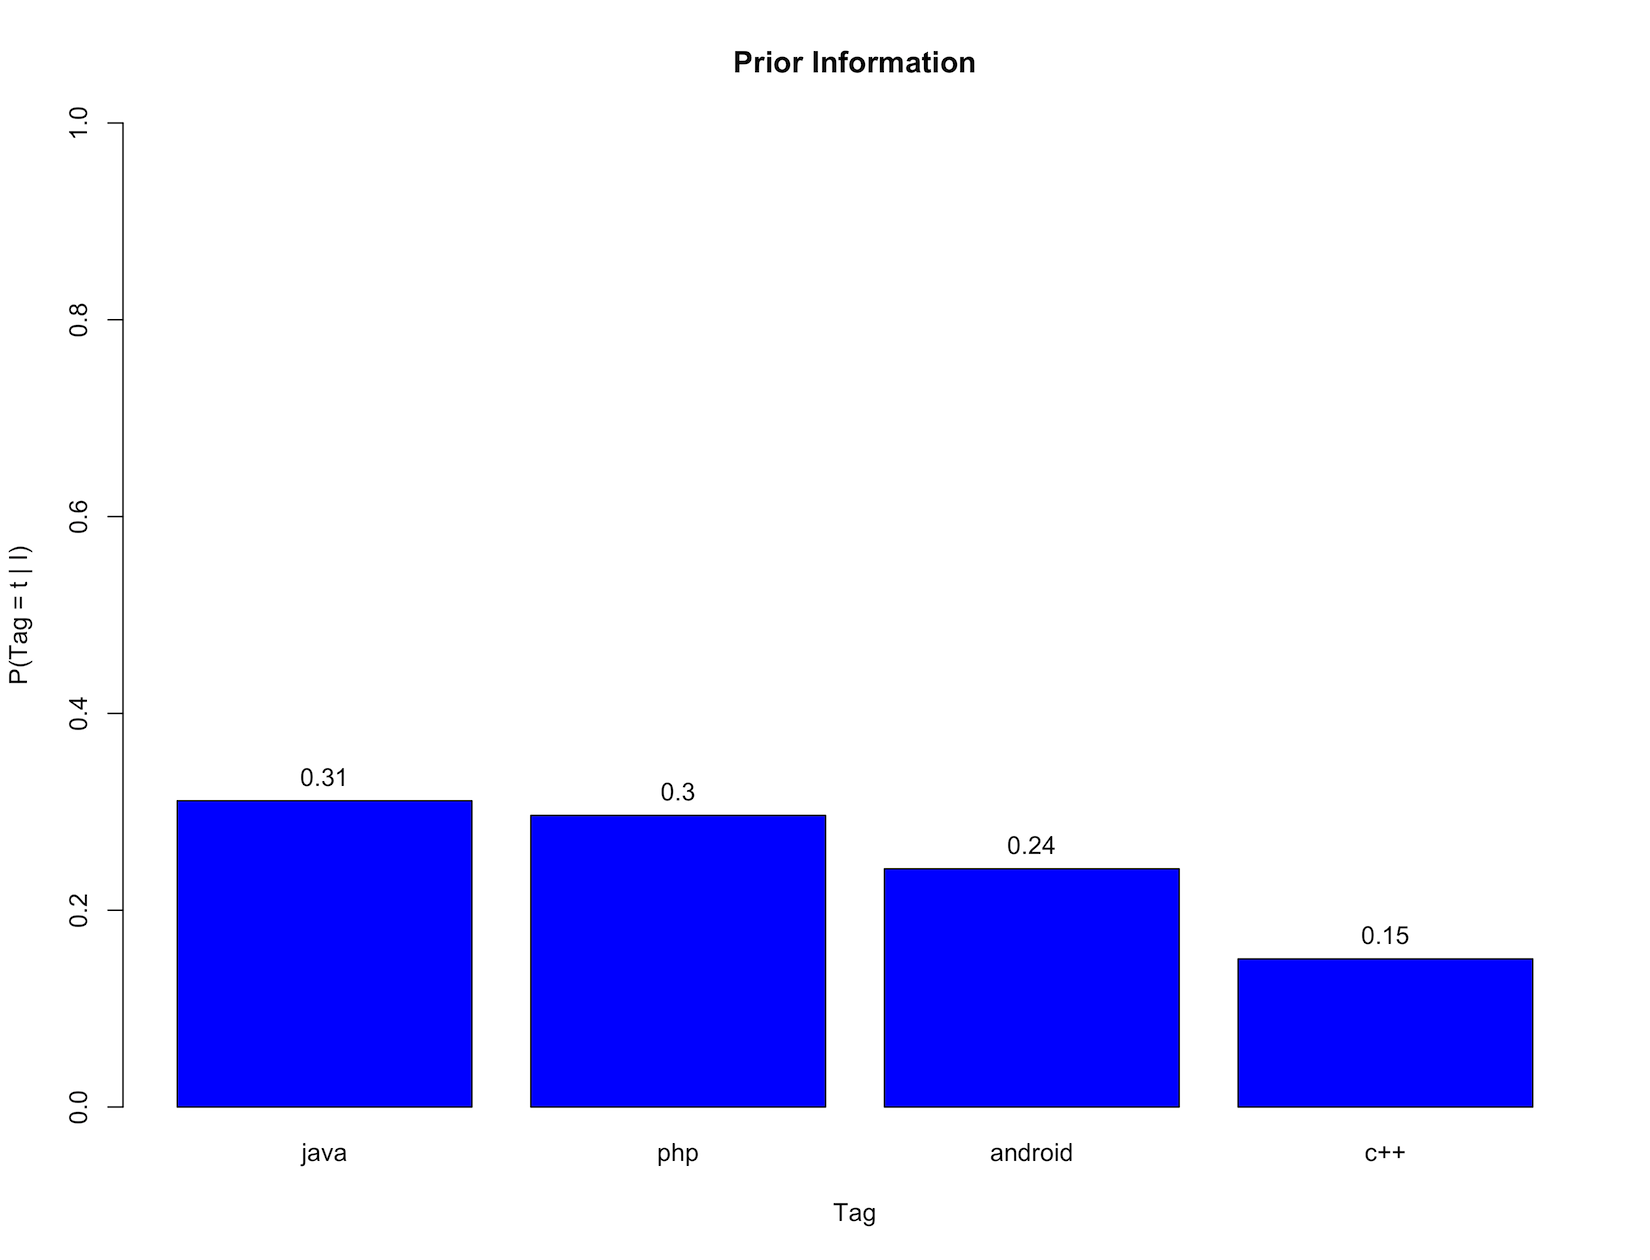
\includegraphics[scale=0.4]{prior}
    \caption{Prior Information}
    \label{fig:prior}
\end{figure}

\begin{figure}[H]
    \centering
    \begin{subfigure}[b]{.40\textwidth}
        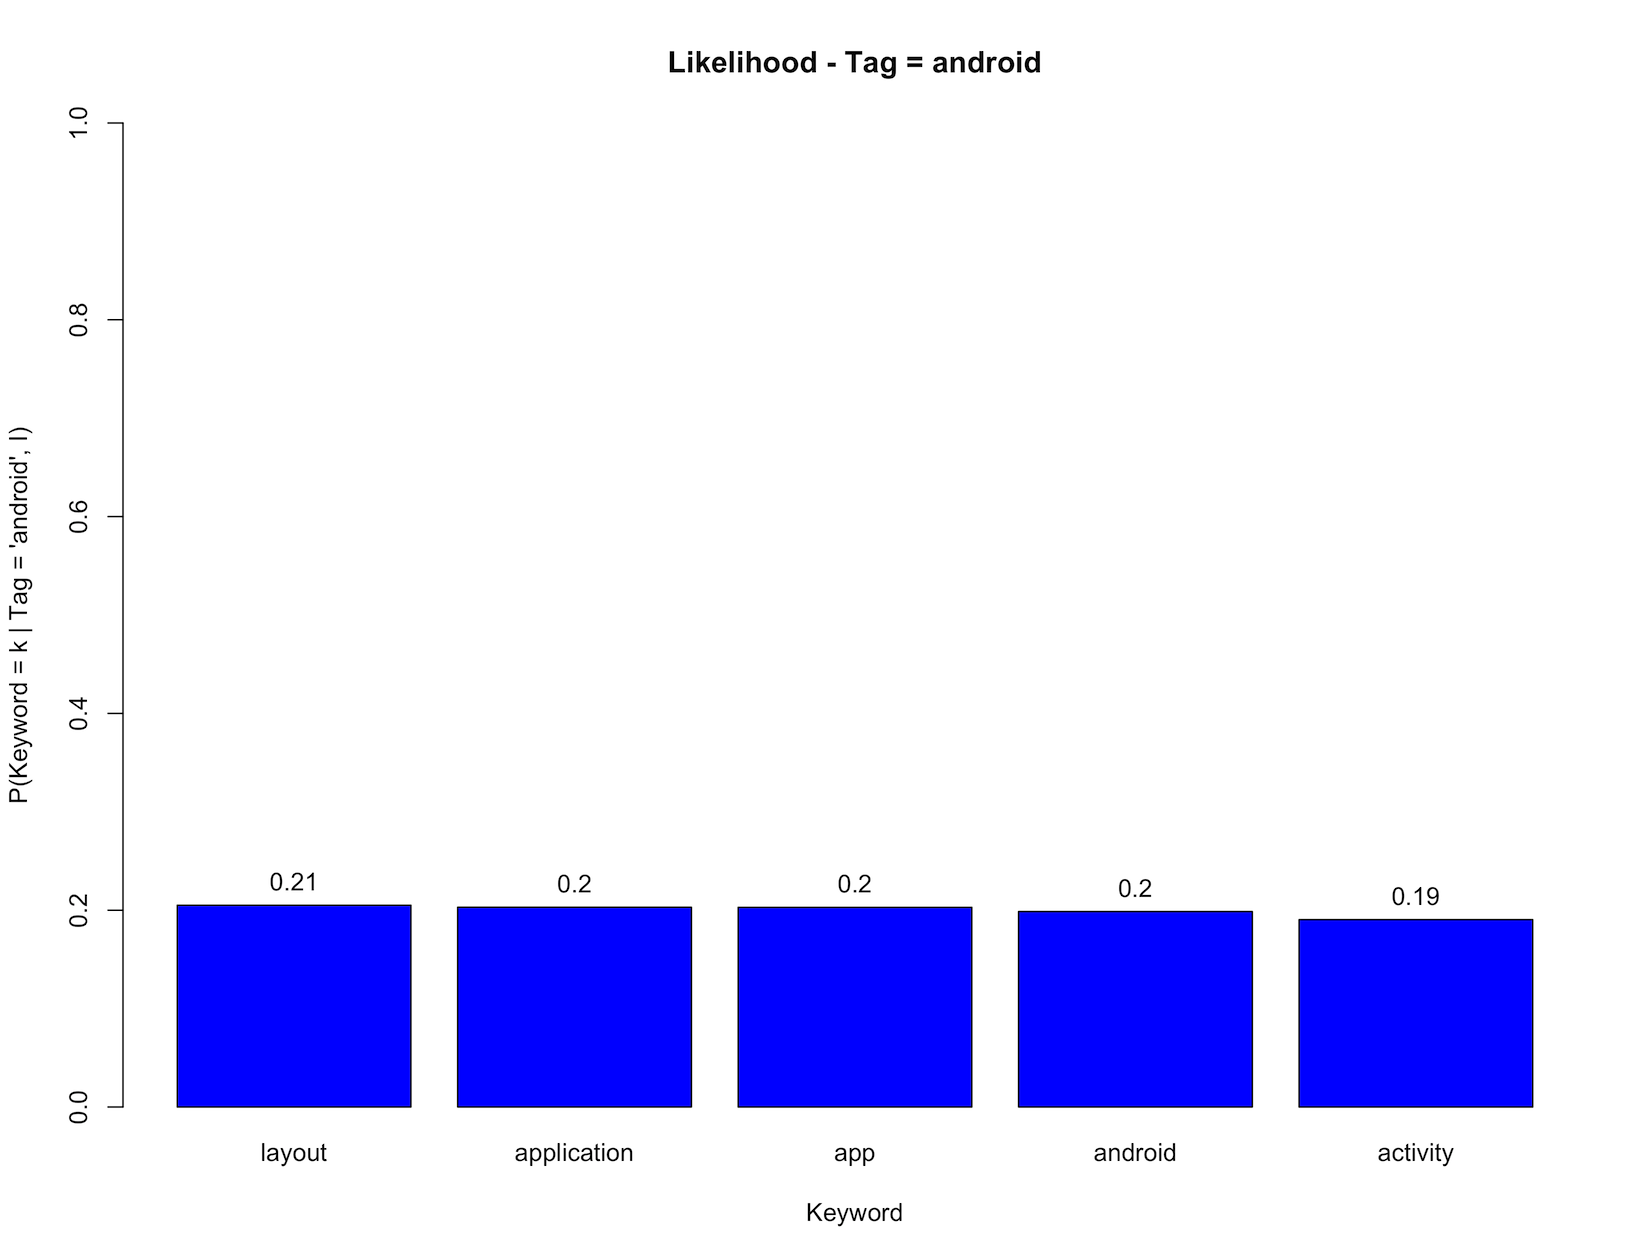
\includegraphics[width=\textwidth]{likelihood_android}
        \caption{Likelihood Android}
        \label{fig:likelihood_android}
    \end{subfigure}
    \begin{subfigure}[b]{.40\textwidth}
        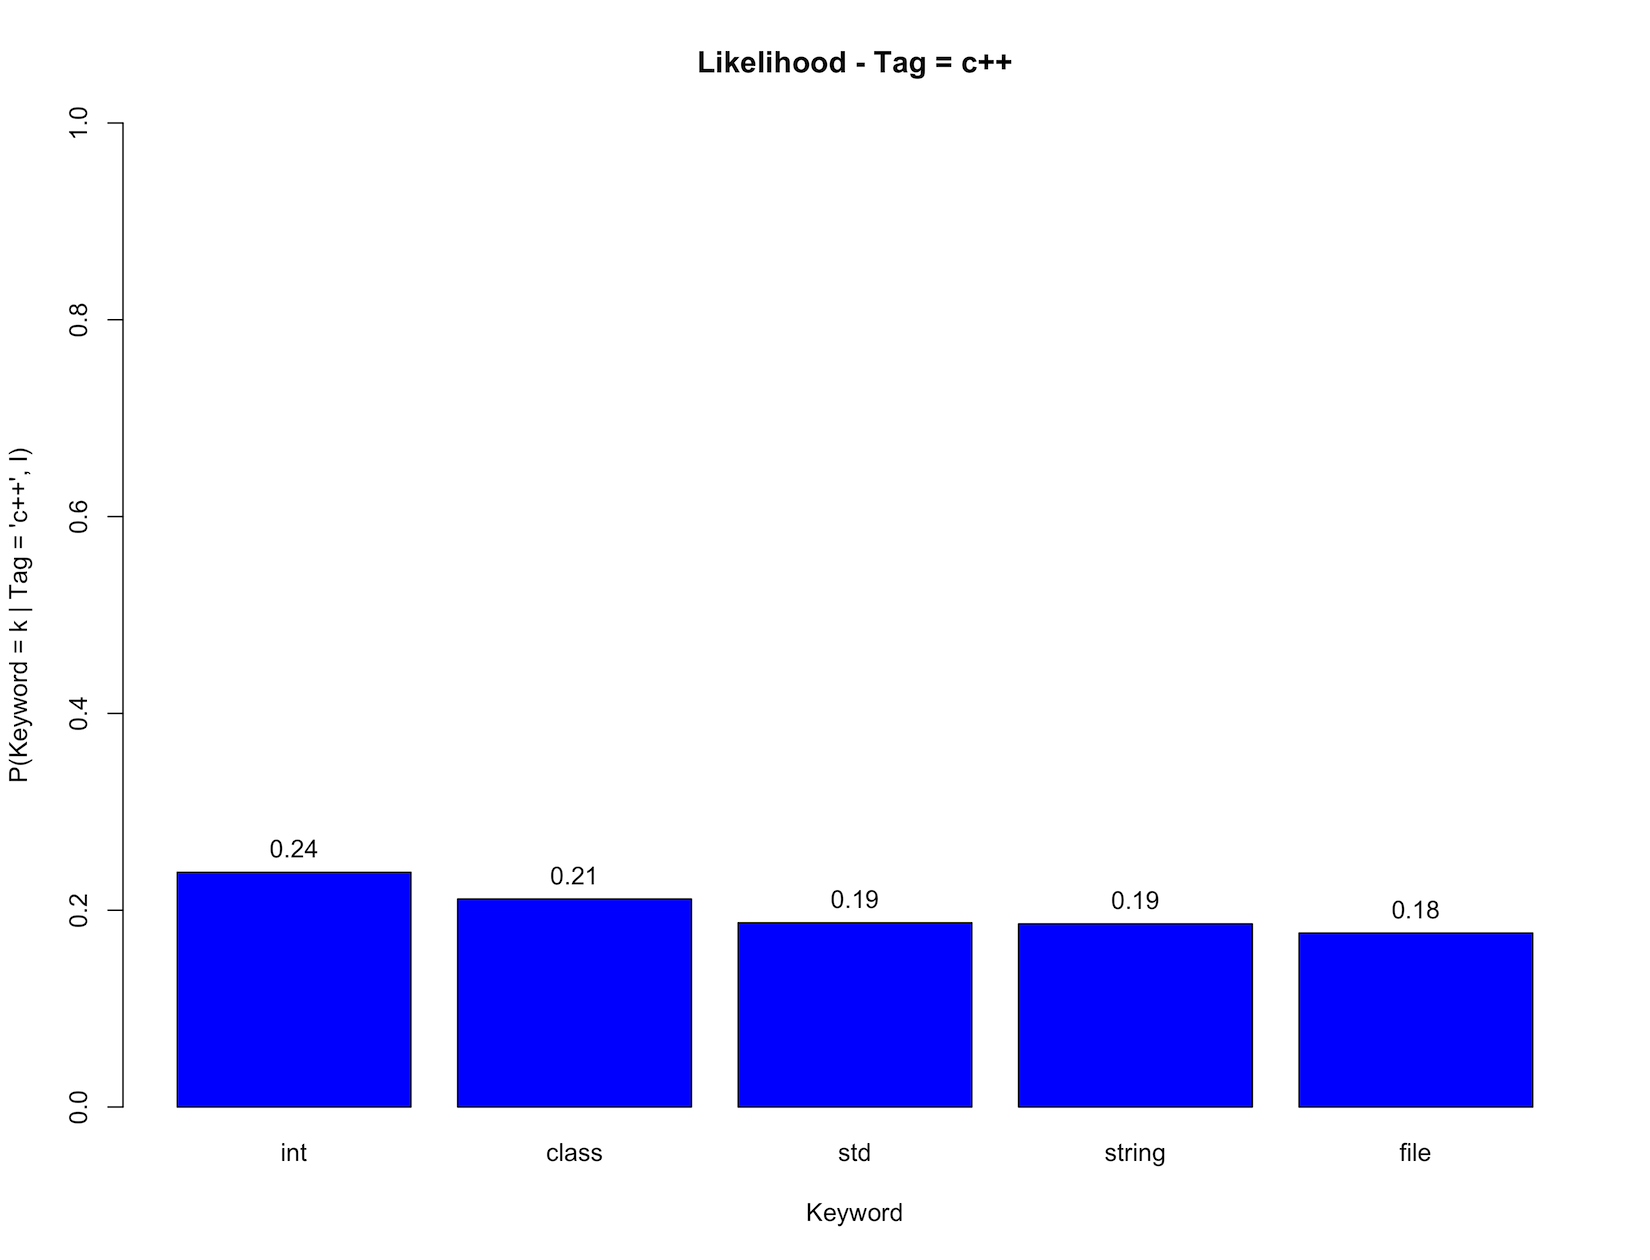
\includegraphics[width=\textwidth]{likelihood_c++}
        \caption{Likelihood C++}
        \label{fig:likelihood_c++}
    \end{subfigure}
    \begin{subfigure}[b]{.40\textwidth}
        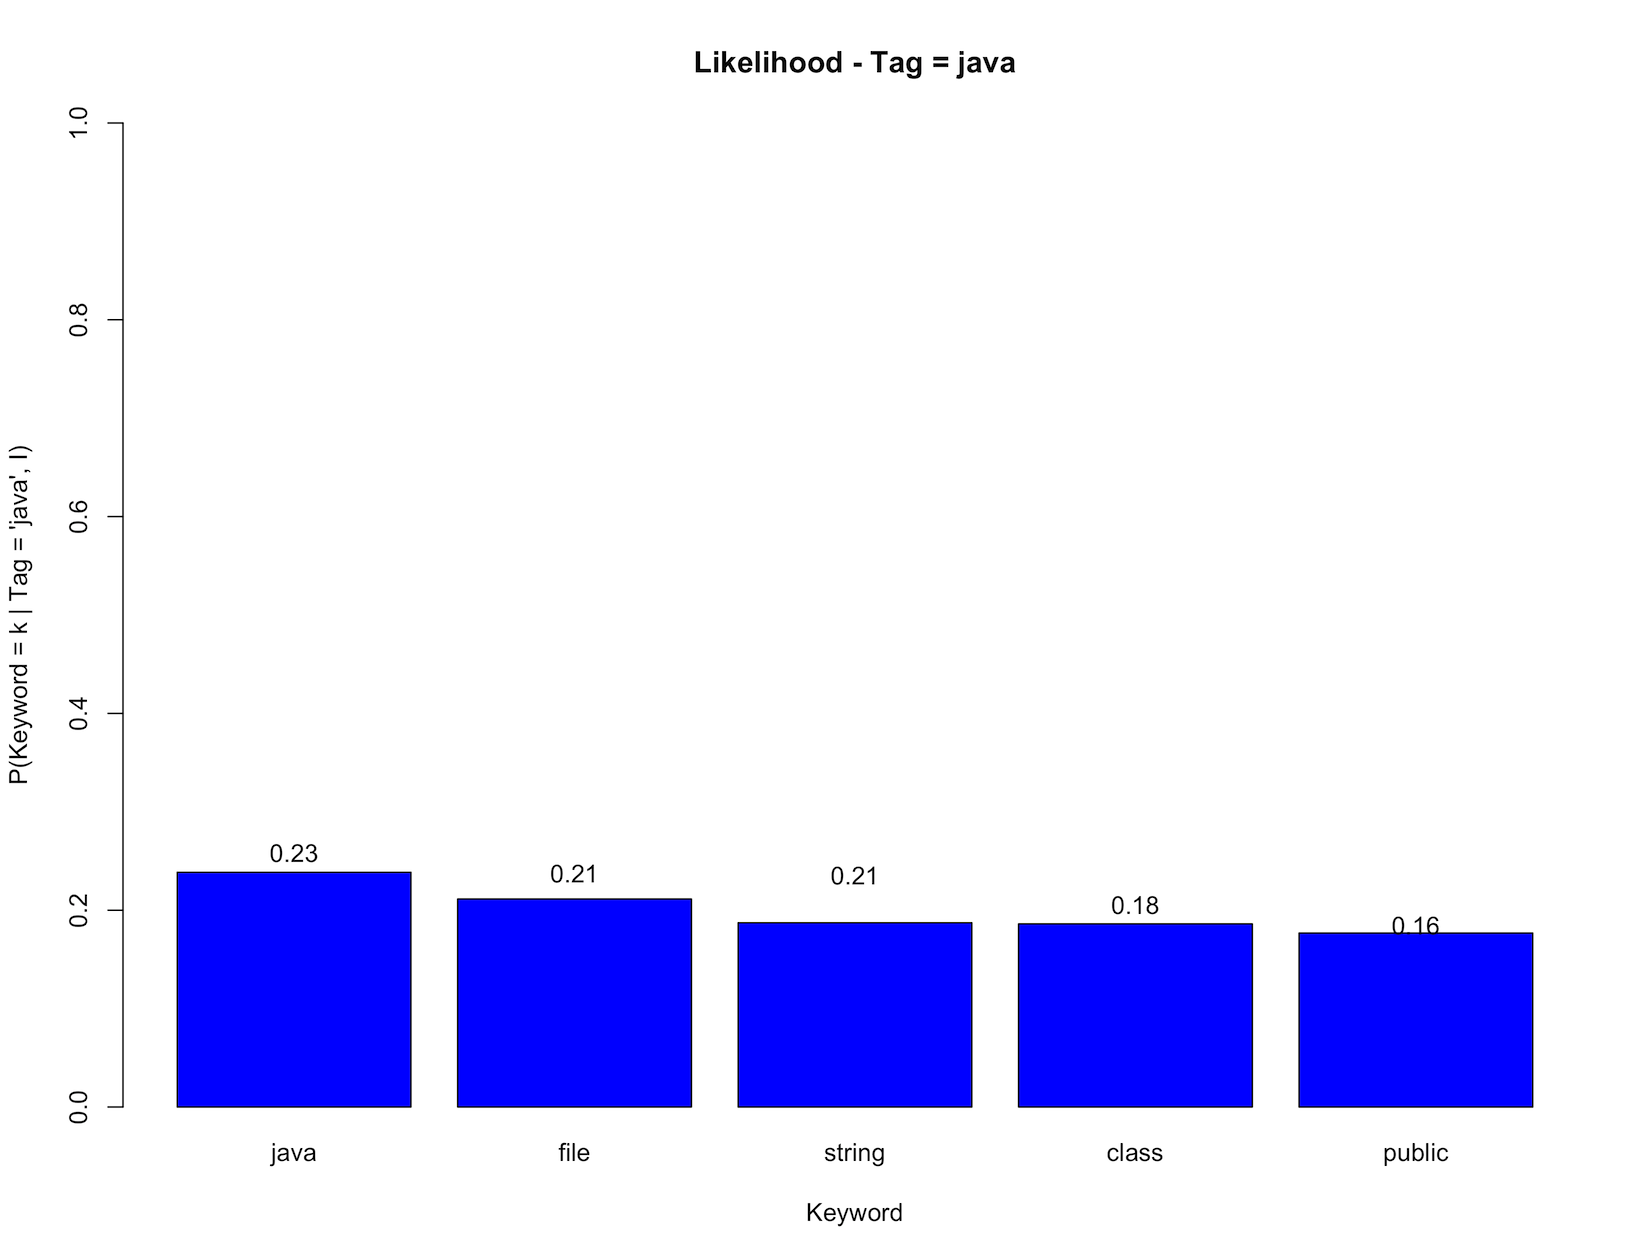
\includegraphics[width=\textwidth]{likelihood_java}
        \caption{Likelihood Java}
        \label{fig:likelihood_java}
    \end{subfigure}
    \begin{subfigure}[b]{.40\textwidth}
        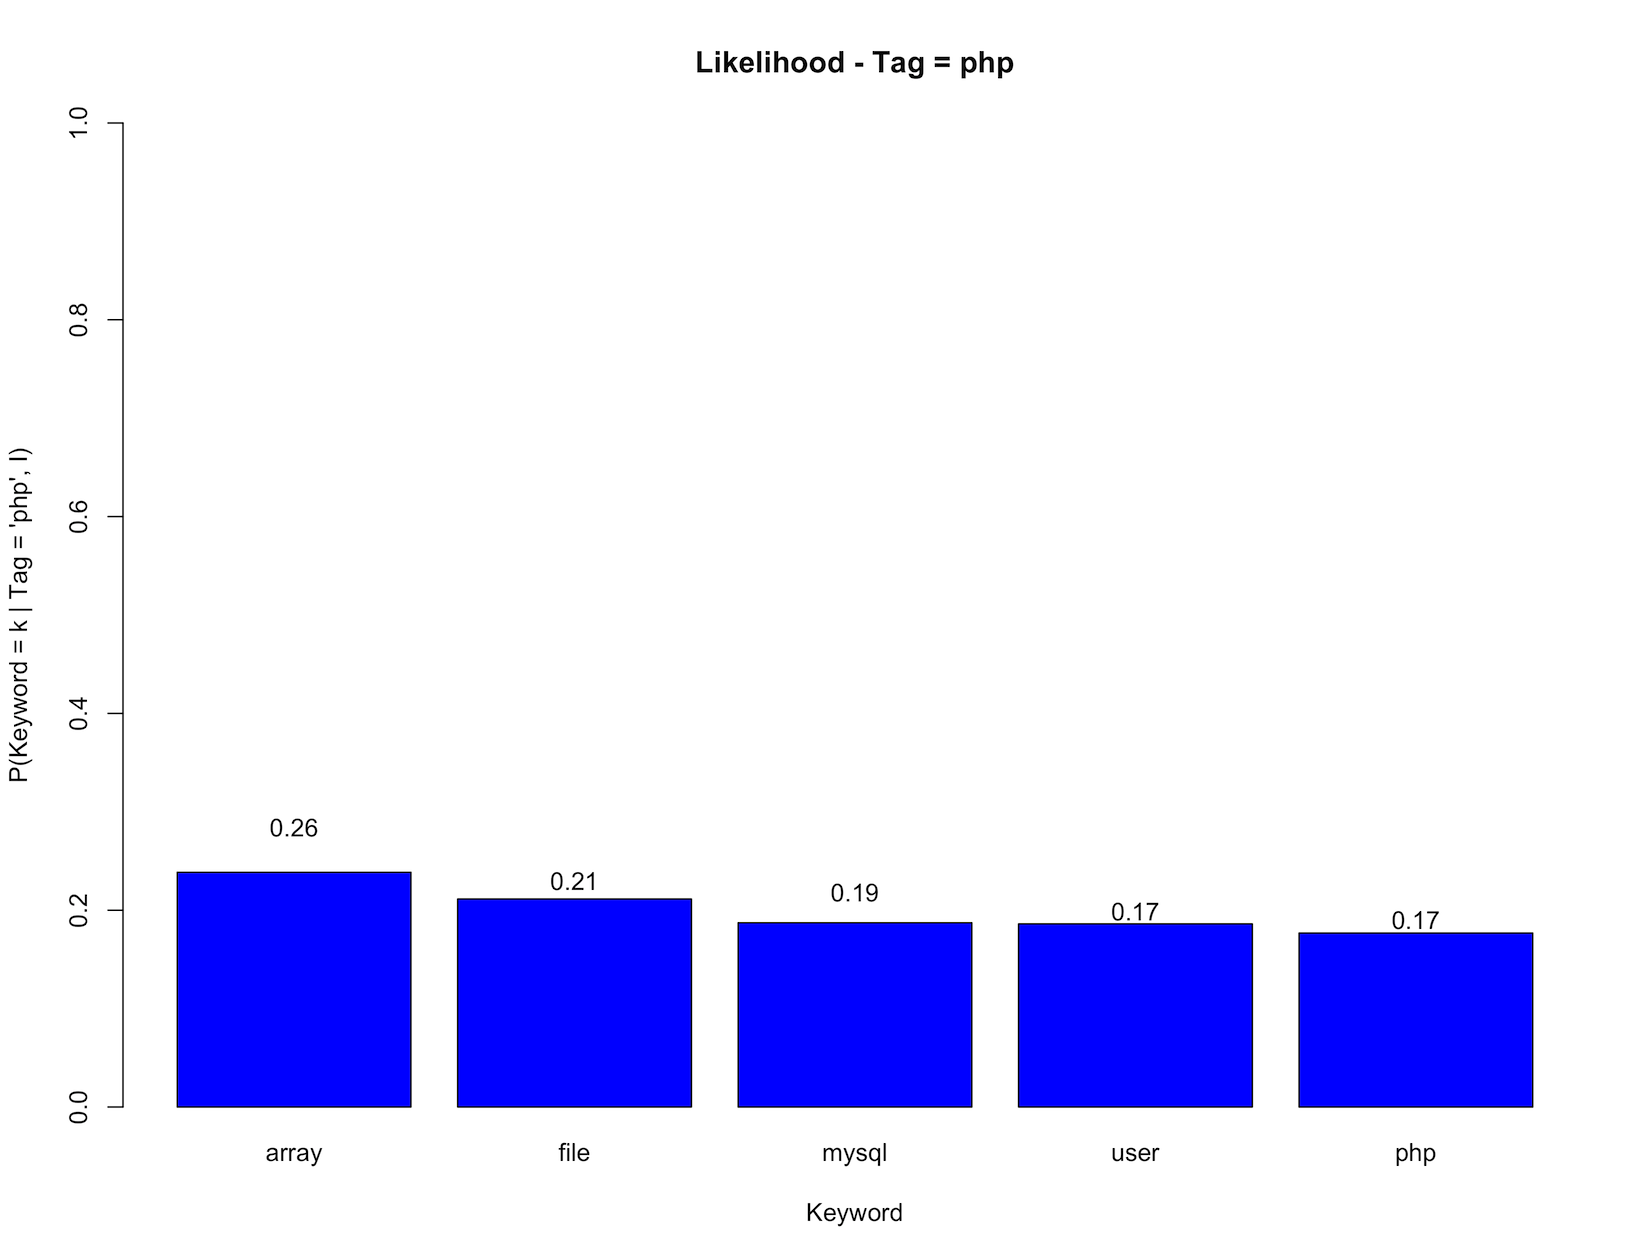
\includegraphics[width=\textwidth]{likelihood_php}
        \caption{Likelihood Php}
        \label{fig:likelihood_php}
    \end{subfigure}
    \caption{Likelihood}
    \label{fig:likelihood}
\end{figure}

\begin{figure}[H]
    \centering
    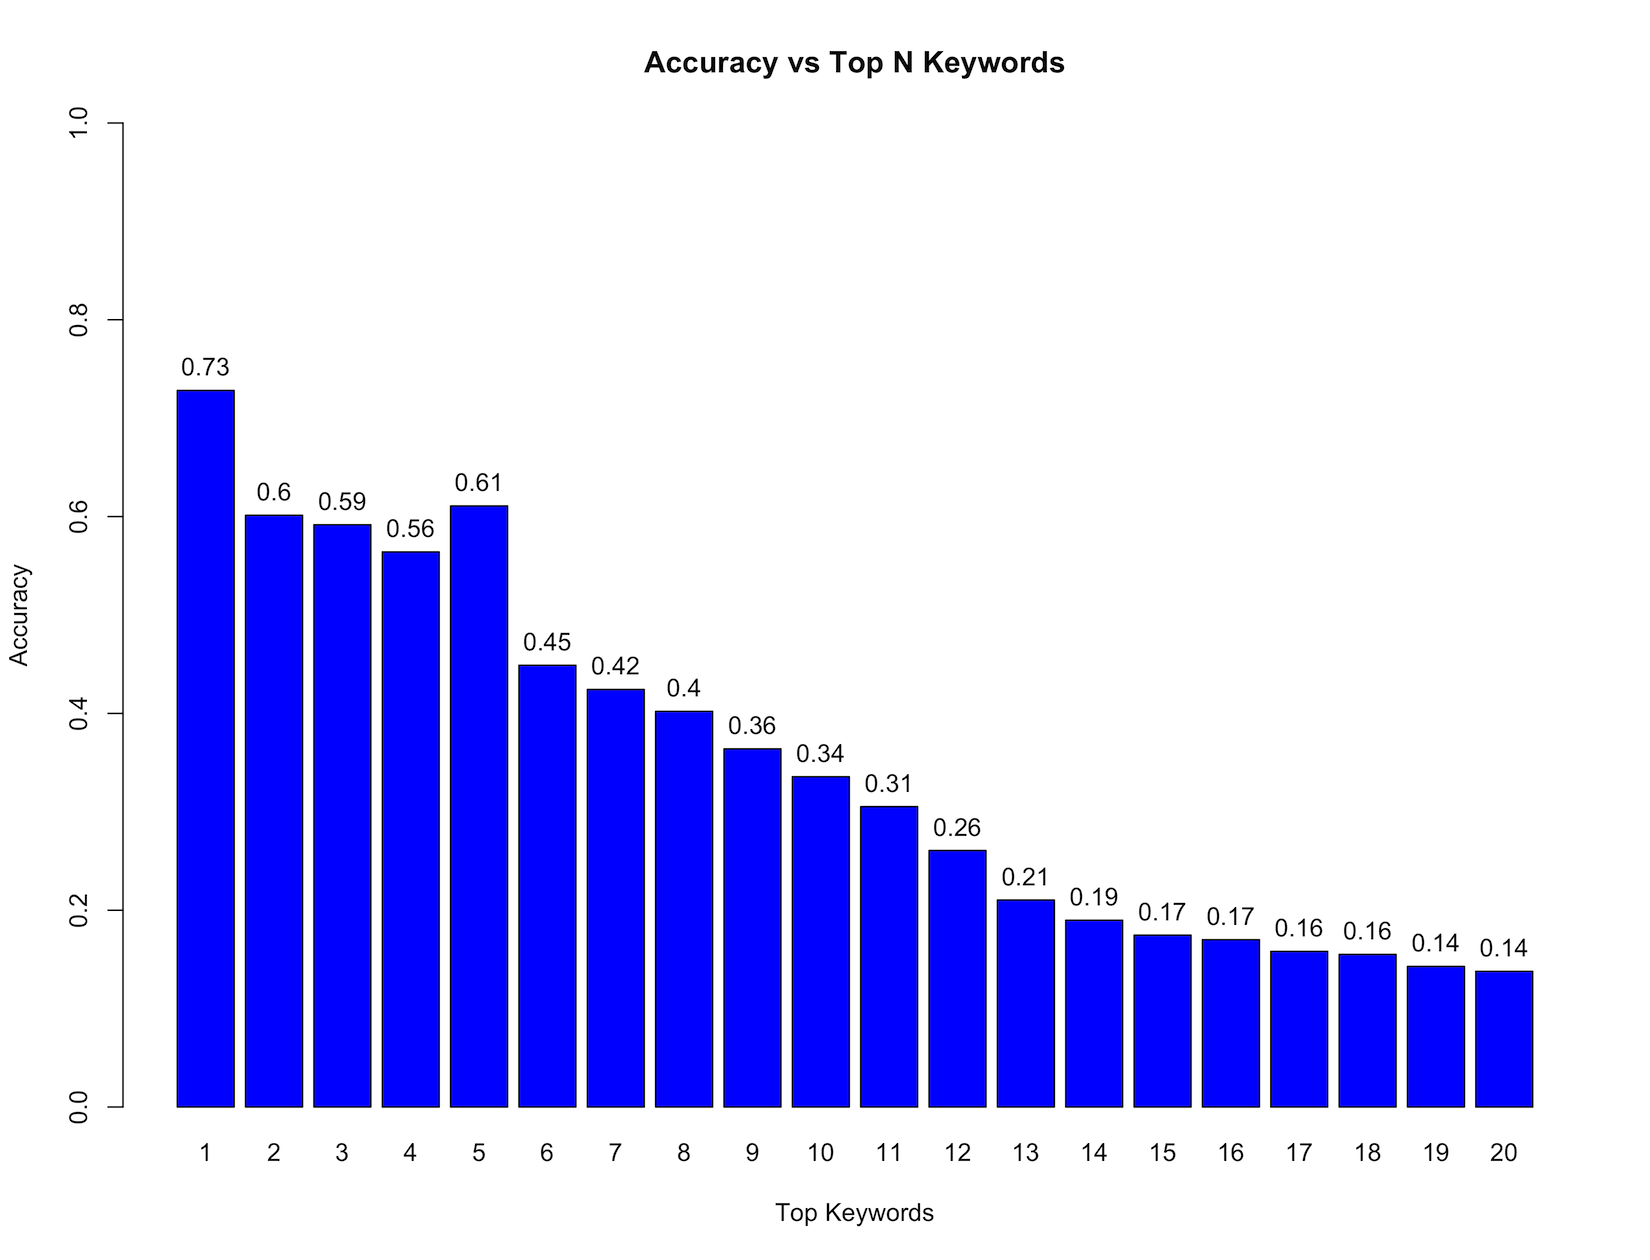
\includegraphics[scale=0.4]{accuracy}
    \caption{Comparison between difference optimization approaches}
    \label{fig:accuracy}
\end{figure}

